%!TEX root = ../report.tex
\documentclass[report.tex]{subfiles}
\begin{document}

    % \chapter{Design Details}
    \chapter{Images}

    \section{Dataset images} \label{appendix:A1}
    Below are some sampled images from dataset \texttt{amy\_gardens}

    \begin{figure}[htbp]
        \centering
        \begin{minipage}[t]{0.32\textwidth}
            \centering
            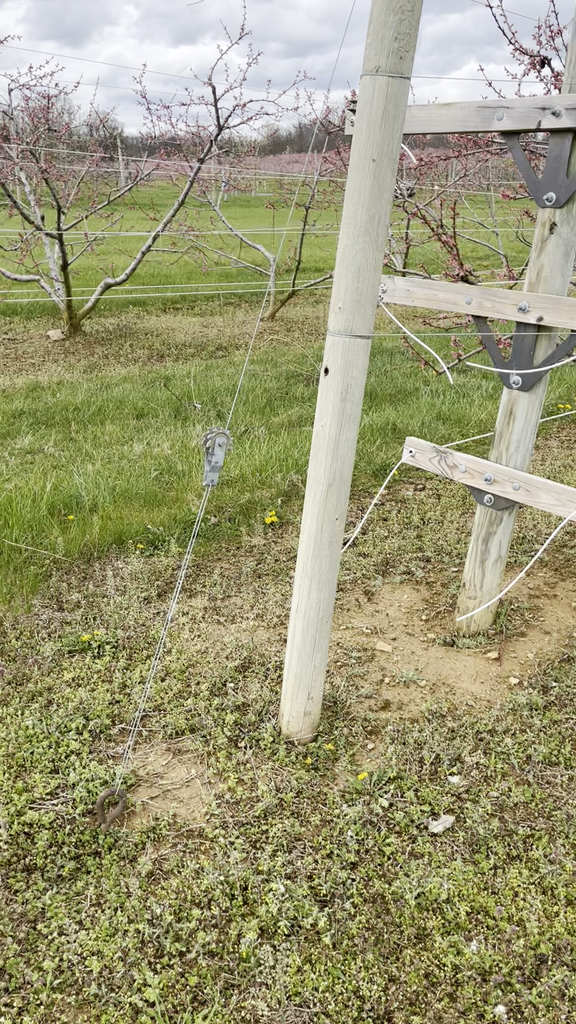
\includegraphics[width=3cm, height=5cm]{images/amy_gardens_dataset/peach_0004.png}
            \subcaption{Image: peach\_0004}
            \label{fig:amygardens1}
        \end{minipage}%
        \hfill
        \begin{minipage}[t]{0.32\textwidth}
            \centering
            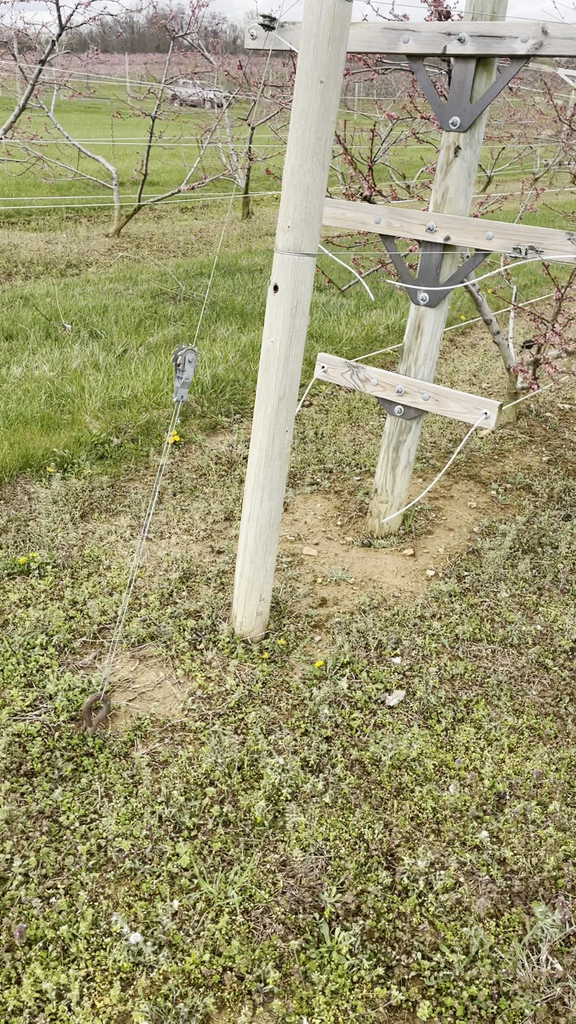
\includegraphics[width=3cm, height=5cm]{images/amy_gardens_dataset/peach_0008.png}
            \subcaption{Image: peach\_0008}
            \label{fig:amygardens2}
        \end{minipage}
        \hfill
        \begin{minipage}[t]{0.32\textwidth}
            \centering
            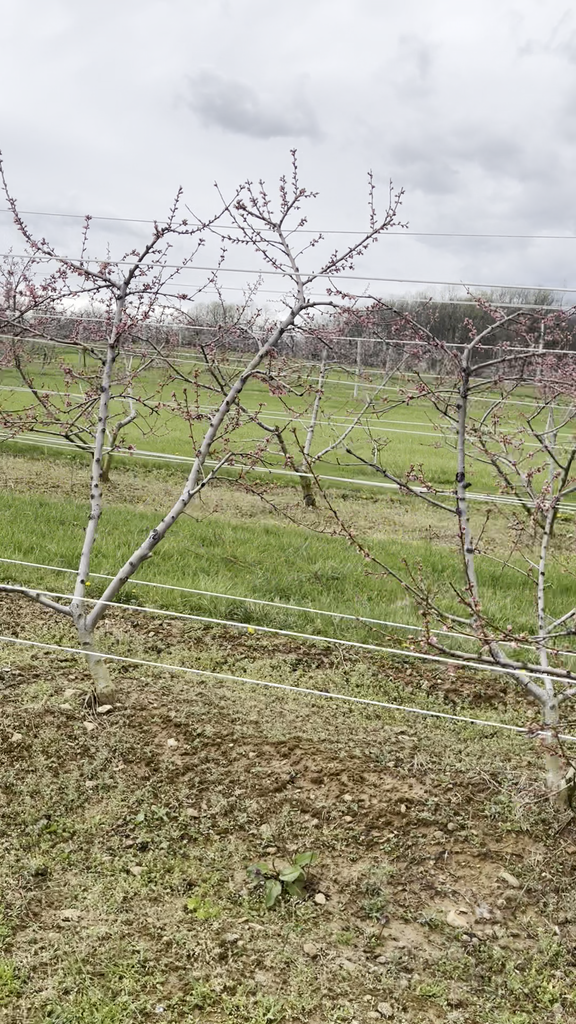
\includegraphics[width=3cm, height=5cm]{images/amy_gardens_dataset/peach_0030.png}
            \subcaption{Image: peach\_0030}
            \label{fig:amygardens3}
        \end{minipage}
    \end{figure}

    \begin{figure}[htbp] \ContinuedFloat
        \centering
        \begin{minipage}[t]{0.32\textwidth}
            \centering
            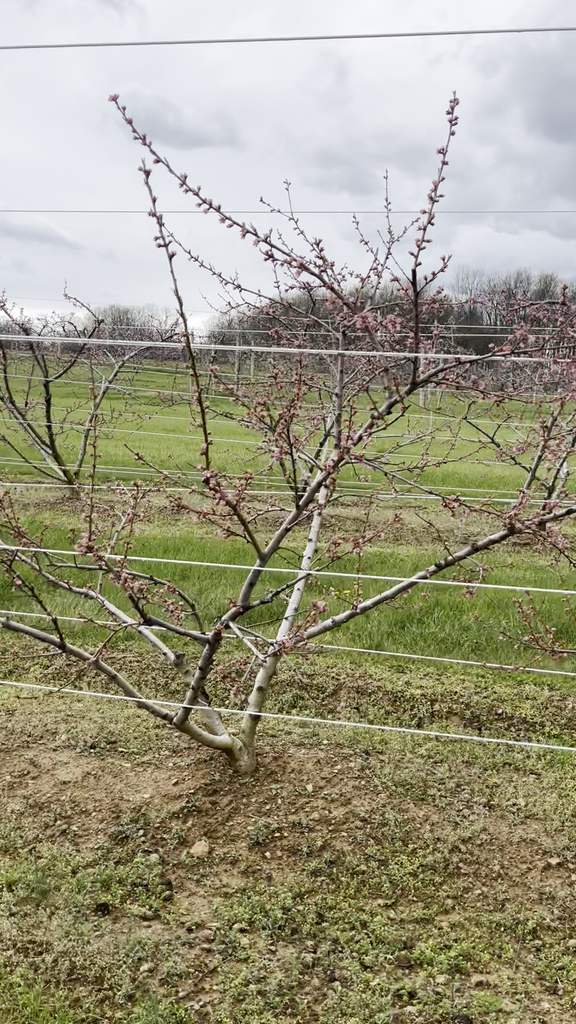
\includegraphics[width=3cm, height=5cm]{images/amy_gardens_dataset/peach_0032.png}
            \subcaption{Image: peach\_0032}
            \label{fig:amygardens4}
        \end{minipage}%
        \hfill
        \begin{minipage}[t]{0.32\textwidth}
            \centering
            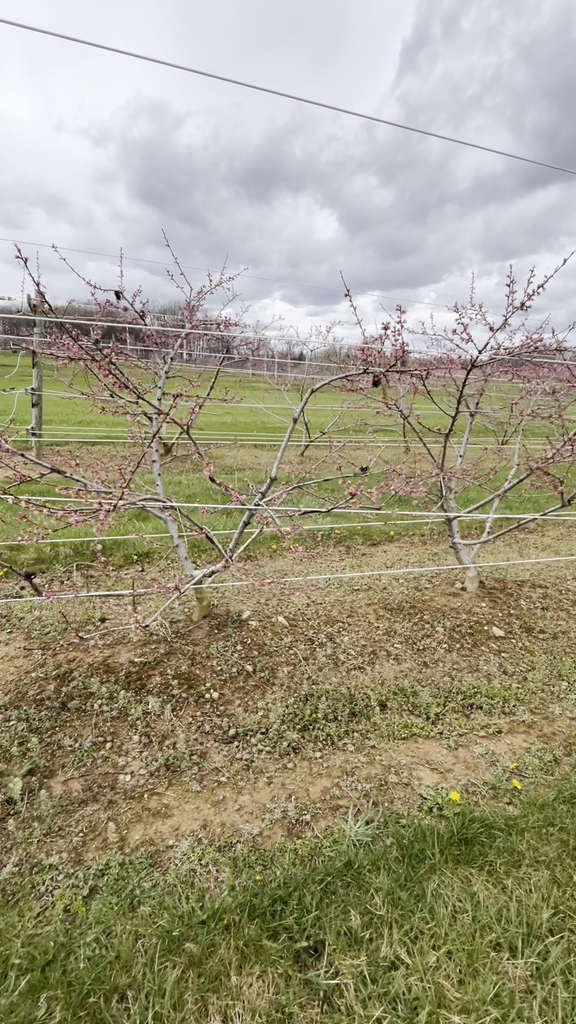
\includegraphics[width=3cm, height=5cm]{images/amy_gardens_dataset/peach_0040.png}
            \subcaption{Image: peach\_0040}
            \label{fig:amygardens5}
        \end{minipage}
        \hfill
        \begin{minipage}[t]{0.32\textwidth}
            \centering
            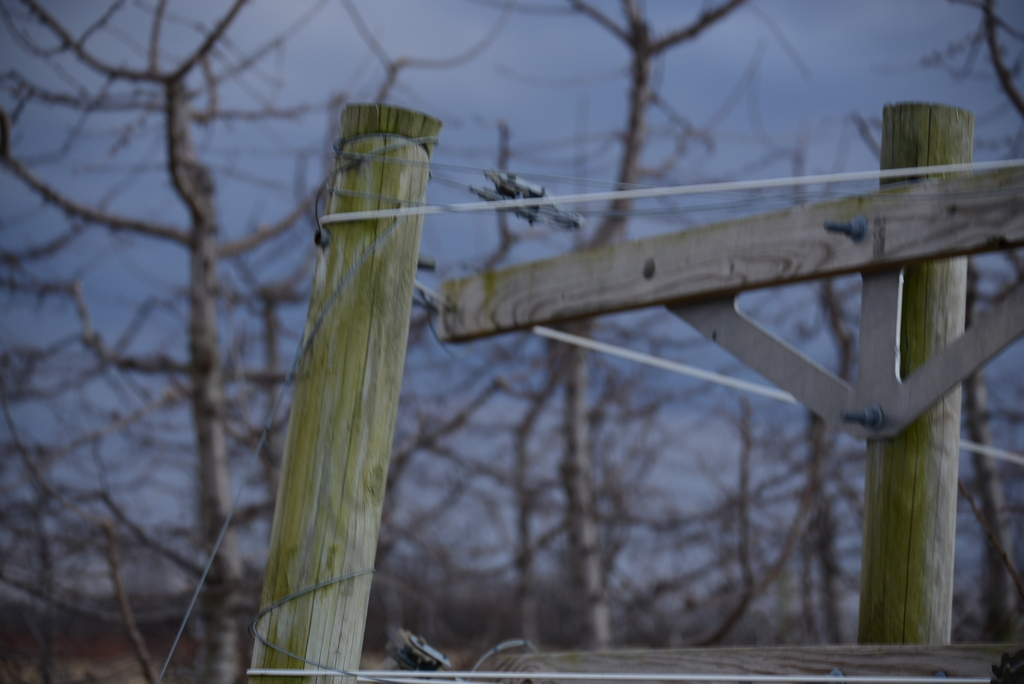
\includegraphics[width=3cm, height=5cm]{images/amy_gardens_dataset/peach_0058.png}
            \subcaption{Image: peach\_0058}
            \label{fig:amygardens6}
        \end{minipage}

        \caption{Different images from the dataset \texttt{amy\_gardens} dataset. The images appear to be highly similar to one another.}
        \label{fig:amygardens_dataset}
    \end{figure}

    \section{Scene-Cluster Overlap Result} \label{appendix:A2}
    The following plots illustrate the scene-cluster overlap for the remaining 9 datasets.

    \begin{figure}[H]
        \centering
        
        \begin{minipage}{\textwidth}
        \centering
        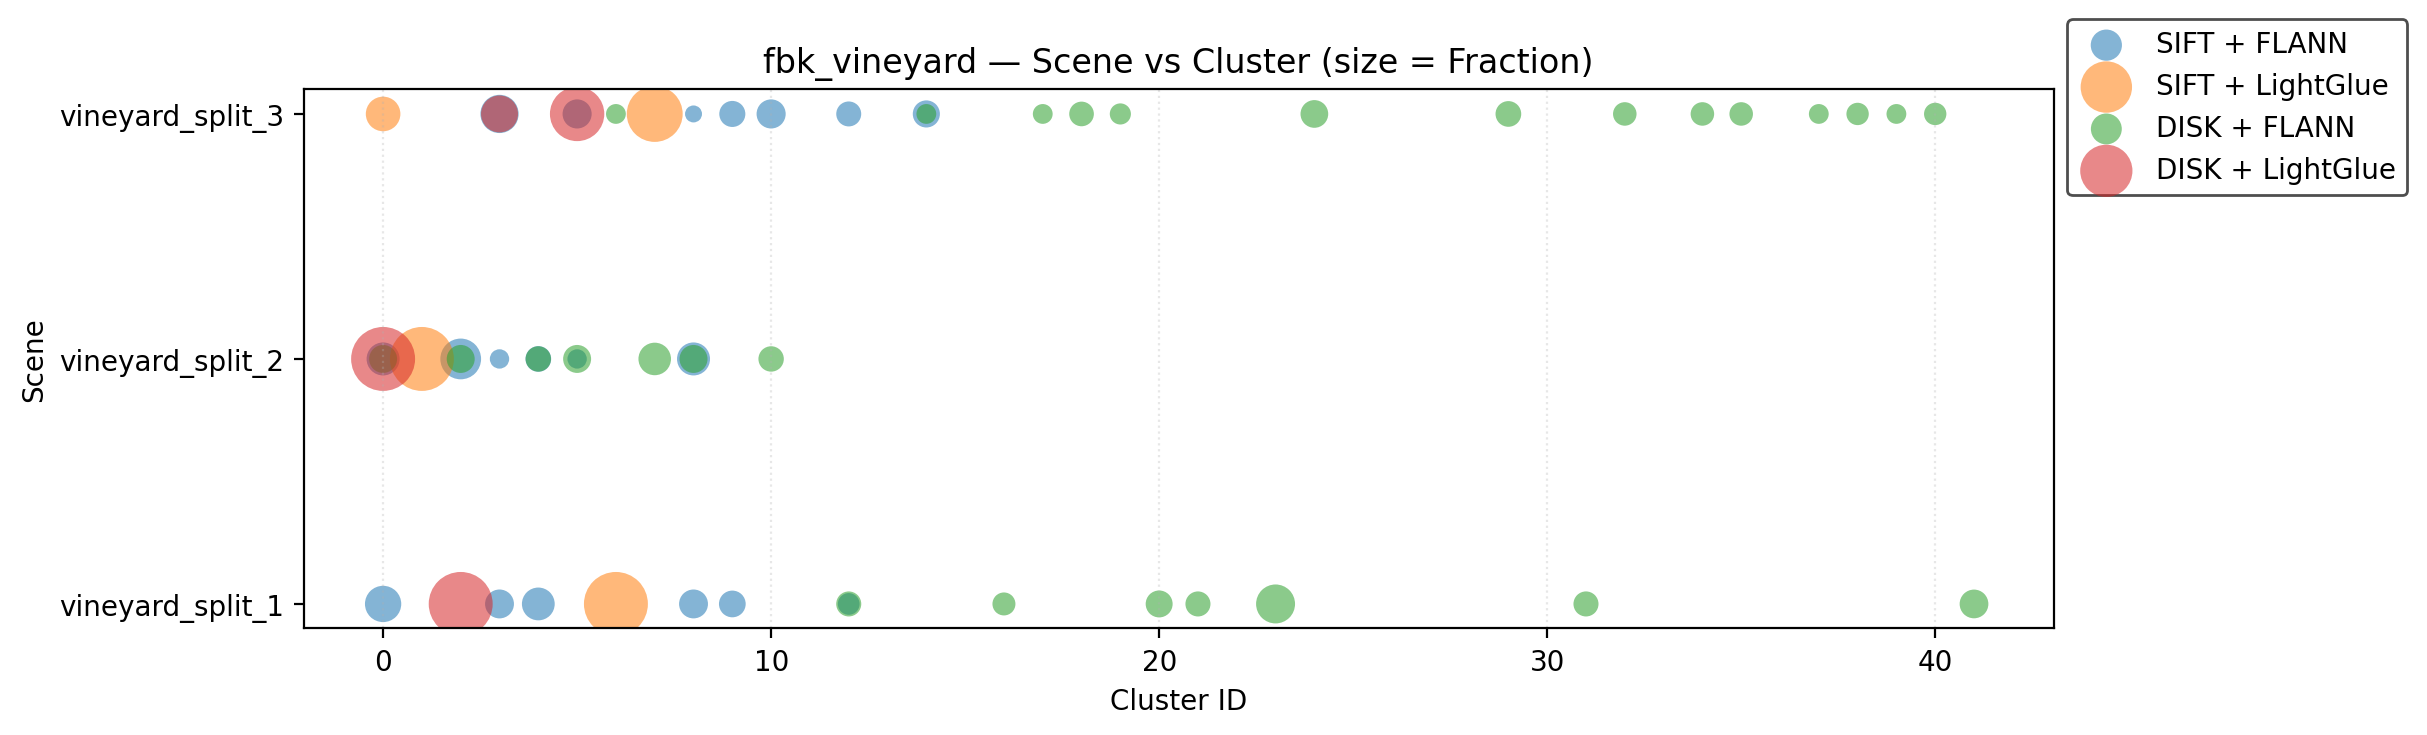
\includegraphics[width=\linewidth]{images/scene_cluster_by_dataset/fbk_vineyard.png}
        \subcaption{Dataset: fbk\_vineyard}
        \label{fig:scene-cluster-A1}
        \end{minipage}\hfill

        \begin{minipage}{\textwidth}
            \centering
            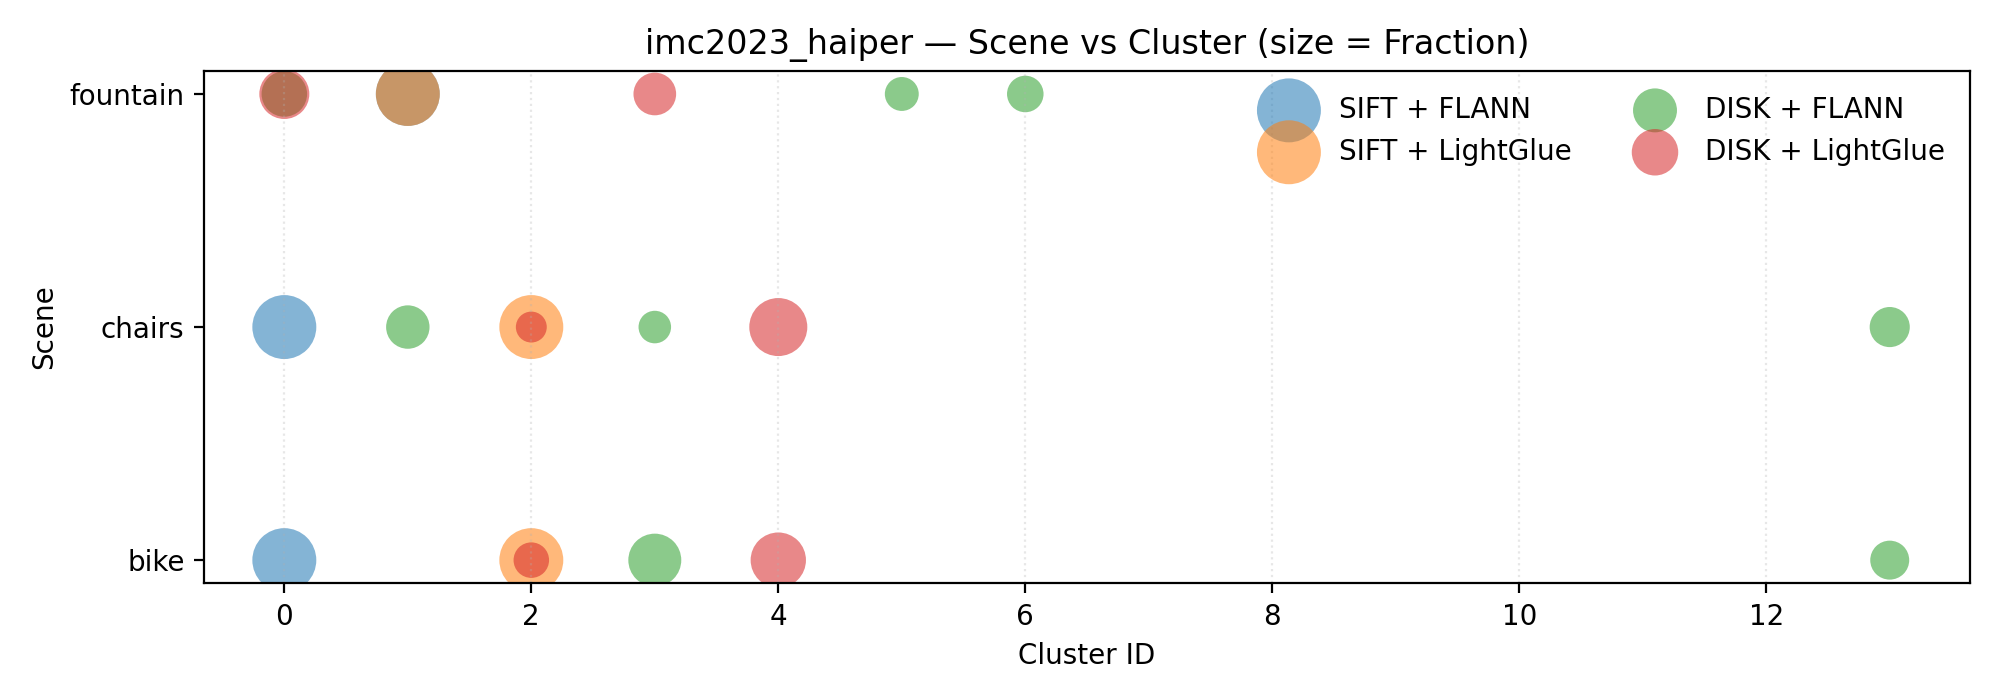
\includegraphics[width=\linewidth]{images/scene_cluster_by_dataset/imc2023_haiper.png}
            \subcaption{Dataset: imc2023\_haiper}
            \label{fig:scene-cluster-A2}
        \end{minipage}\hfill
    
        \begin{minipage}{\textwidth}
            \centering
            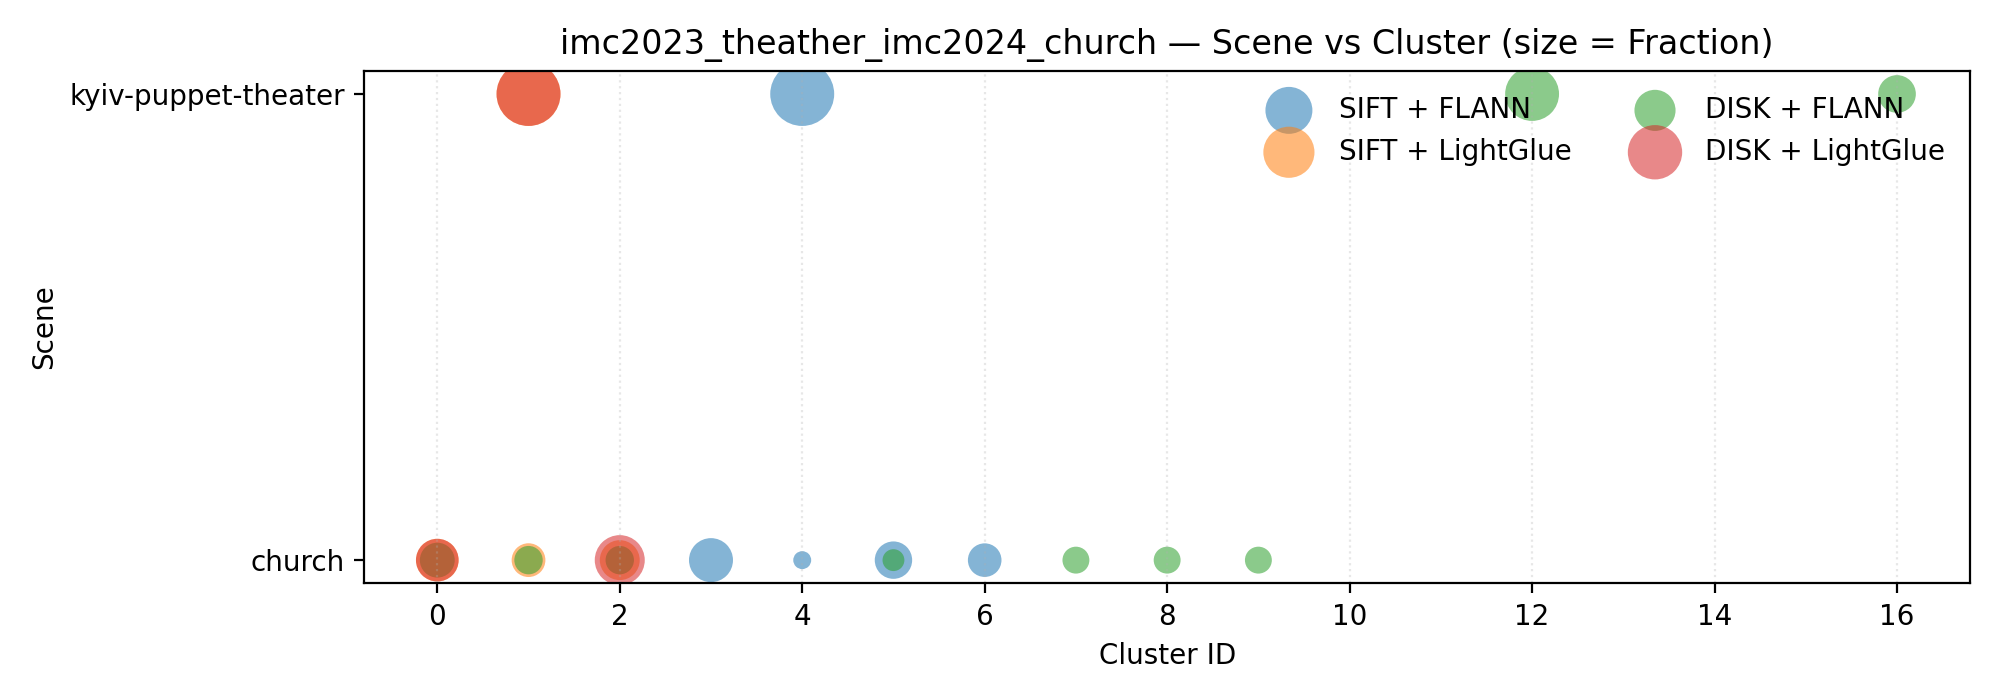
\includegraphics[width=\linewidth]{images/scene_cluster_by_dataset/imc2023_theather_imc2024_church.png}
            \subcaption{Dataset: imc2023\_theather\_imc2024\_church}
            \label{fig:scene-cluster-A3}
        \end{minipage}
    \end{figure}

    \begin{figure}\ContinuedFloat
        \begin{minipage}{\textwidth}
            \centering
            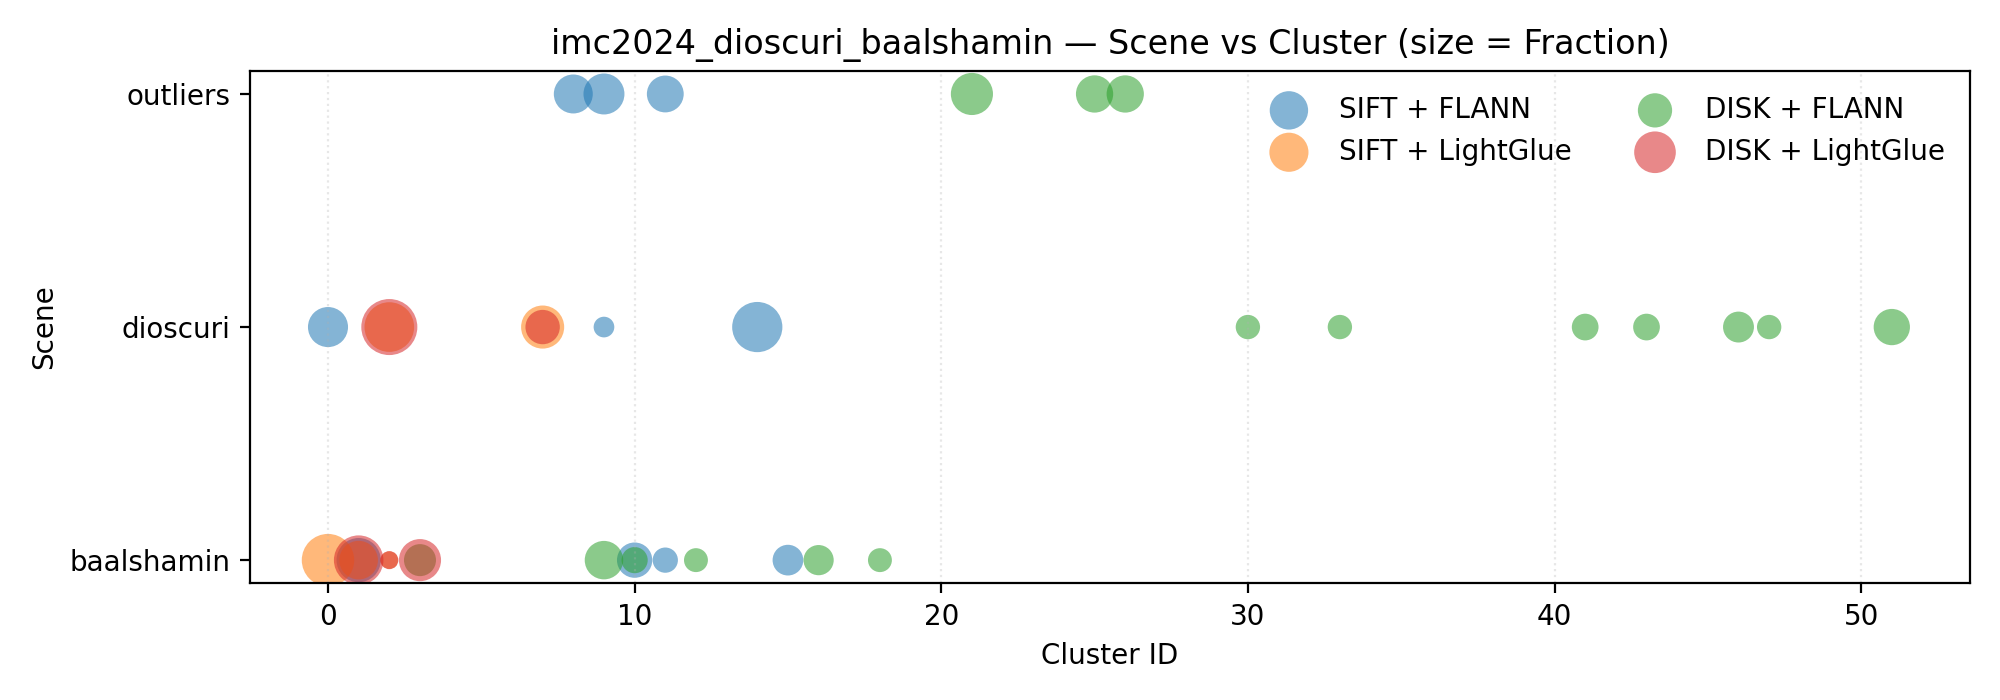
\includegraphics[width=\linewidth]{images/scene_cluster_by_dataset/imc2024_dioscuri_baalshamin.png}
            \subcaption{Dataset: imc2024\_dioscuri\_baalshamin}
            \label{fig:scene-cluster-A4}
        \end{minipage}

        \begin{minipage}{\textwidth}
            \centering
            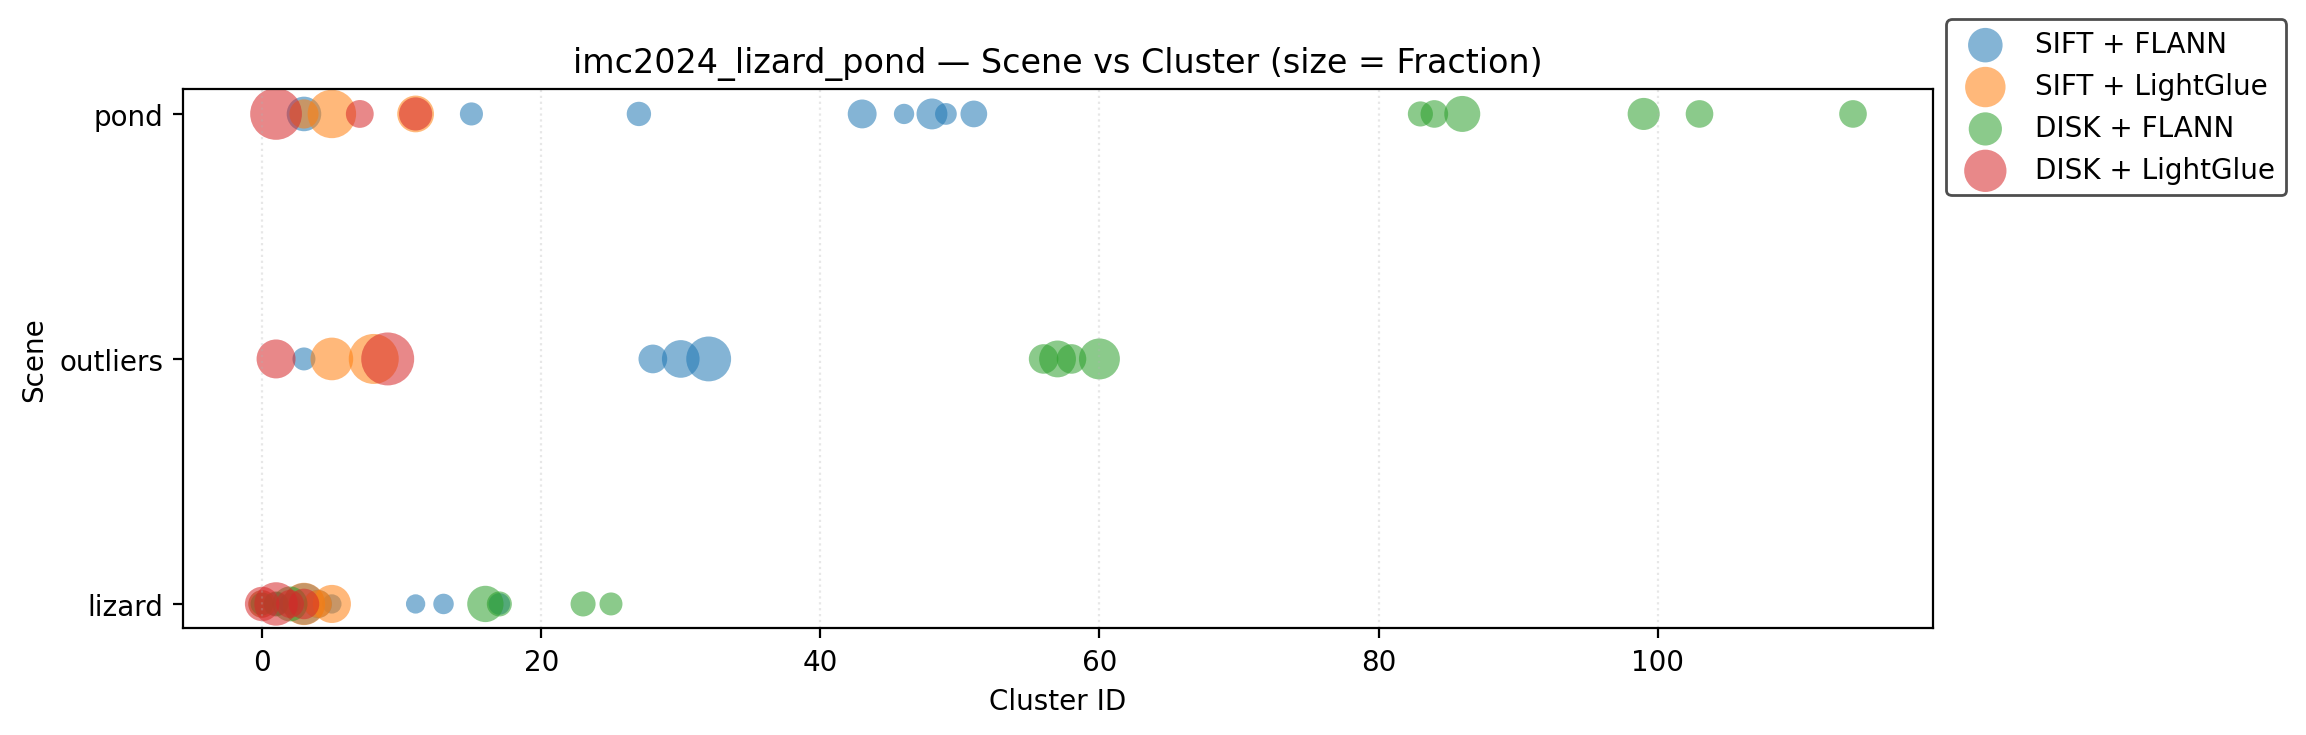
\includegraphics[width=\linewidth]{images/scene_cluster_by_dataset/imc2024_lizard_pond.png}
            \subcaption{Dataset: imc2024\_lizard\_pond}
            \label{fig:scene-cluster-A5}
        \end{minipage}

        \begin{minipage}{\textwidth}
            \centering
            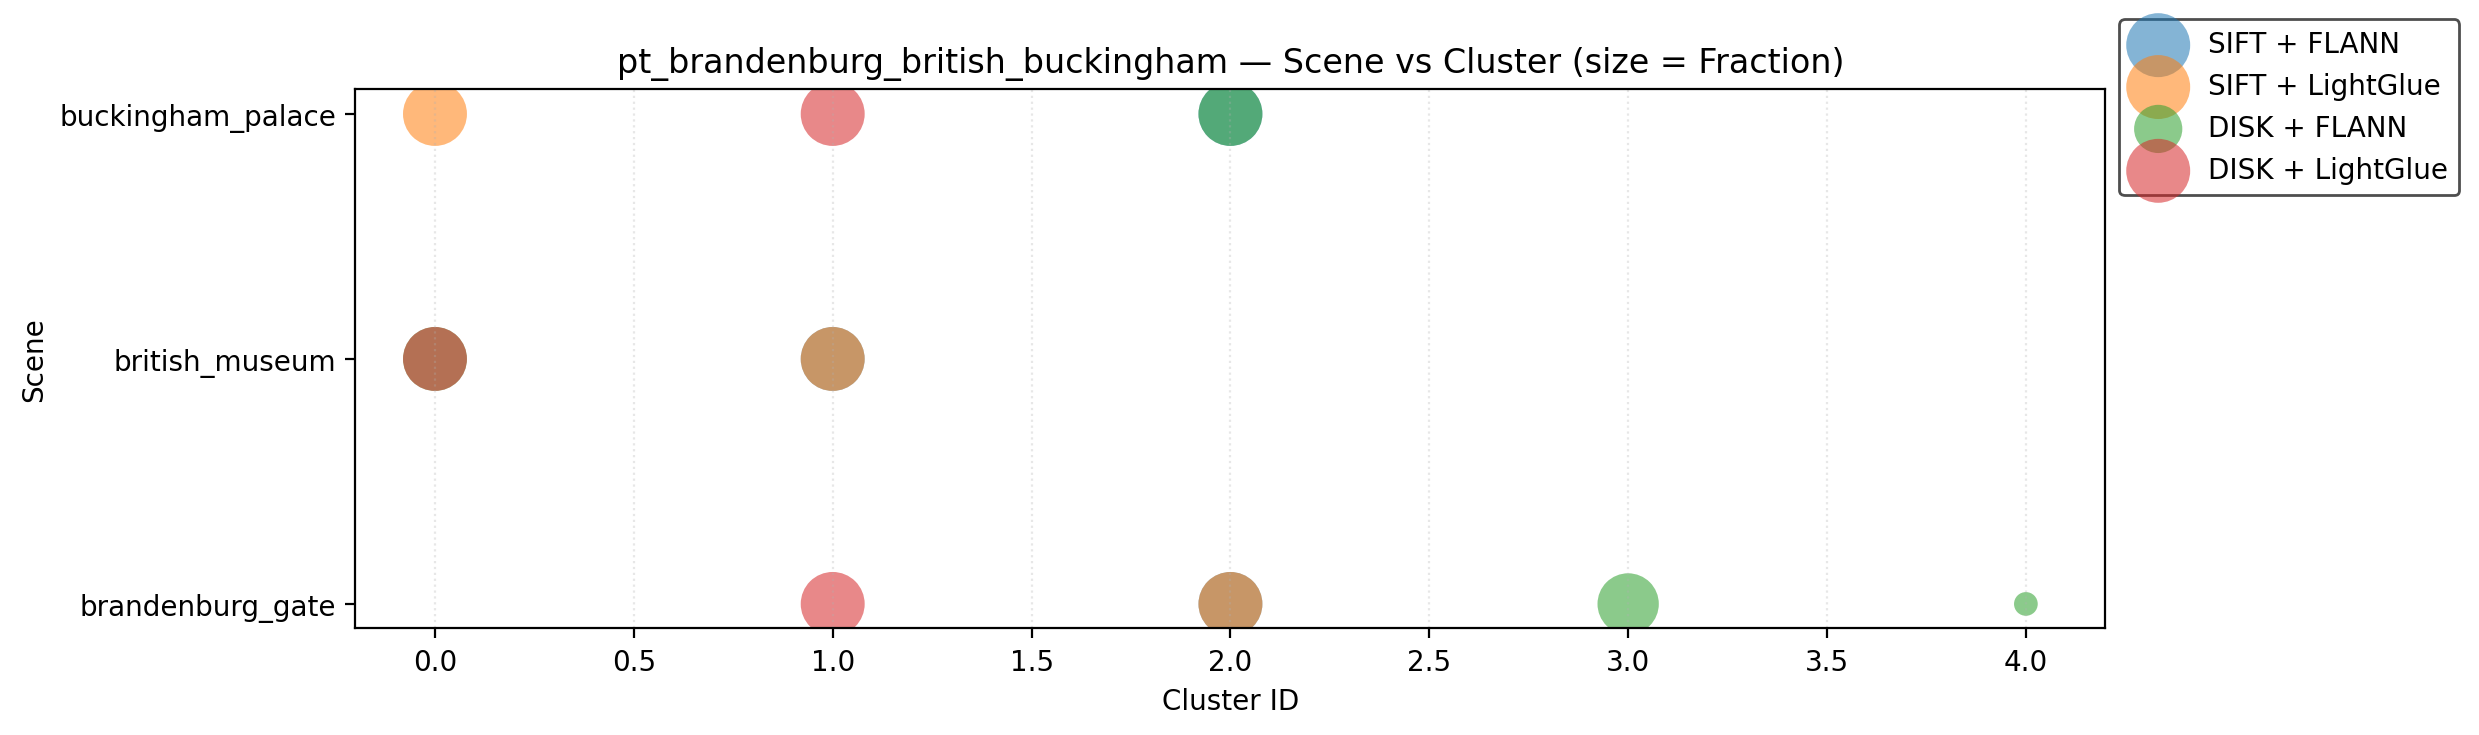
\includegraphics[width=\linewidth]{images/scene_cluster_by_dataset/pt_brandenburg_british_buckingham.png}
            \subcaption{Dataset: pt\_brandenburg\_british\_buckingham}
            \label{fig:scene-cluster-A6}
        \end{minipage}
    \end{figure}

    \begin{figure}[htbp]\ContinuedFloat
        \begin{minipage}{\textwidth}
            \centering
            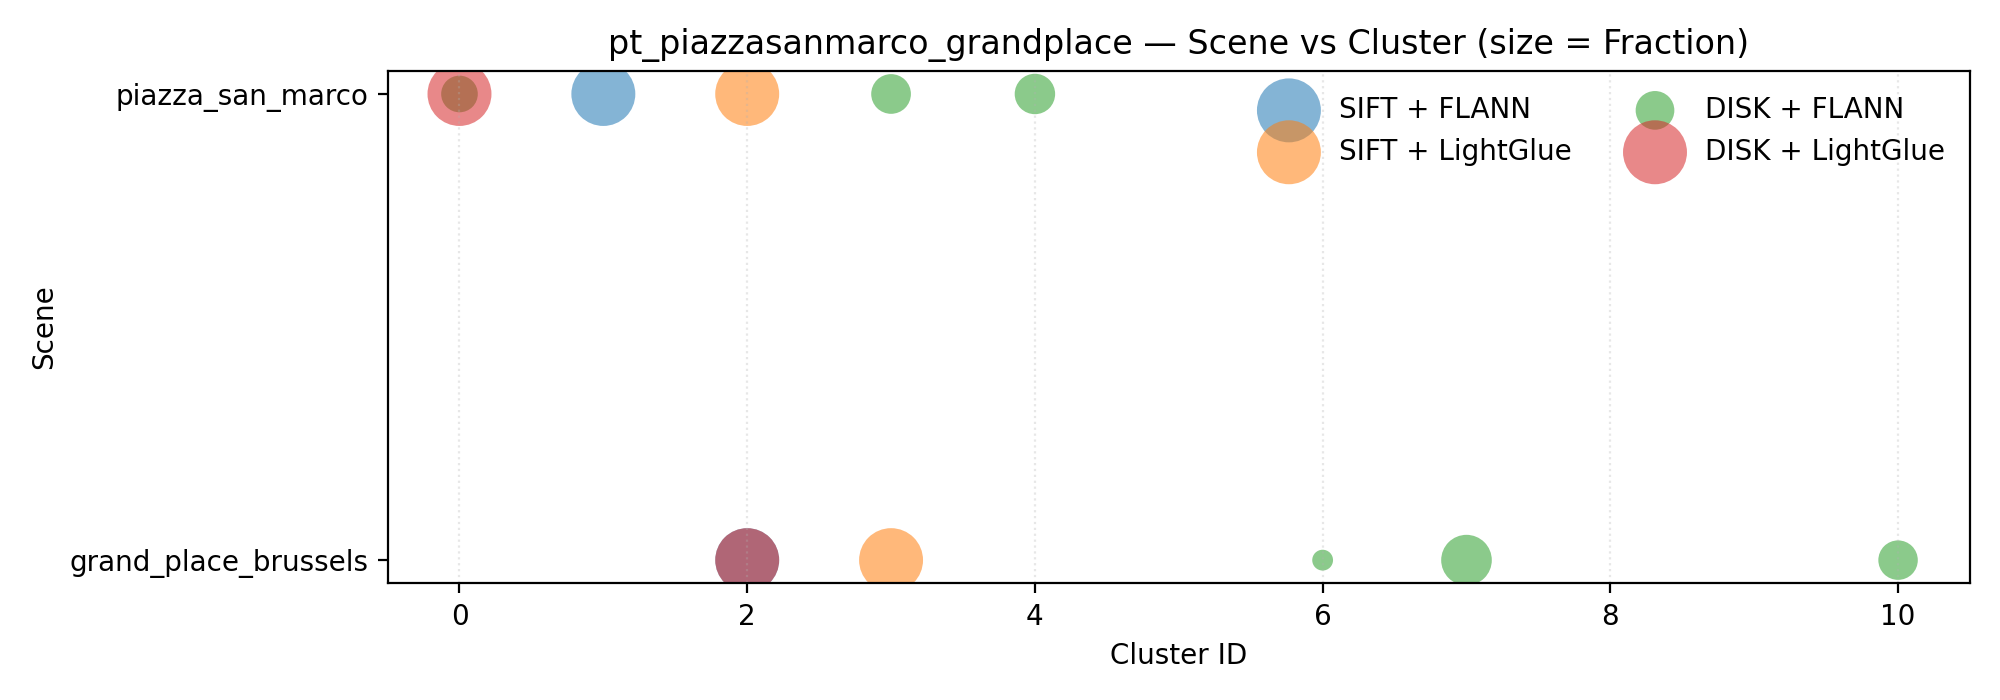
\includegraphics[width=\linewidth]{images/scene_cluster_by_dataset/pt_piazzasanmarco_grandplace.png}
            \subcaption{Dataset: pt\_piazzasanmarco\_grandplace}
            \label{fig:scene-cluster-A7}
        \end{minipage}

        \begin{minipage}{\textwidth}
            \centering
            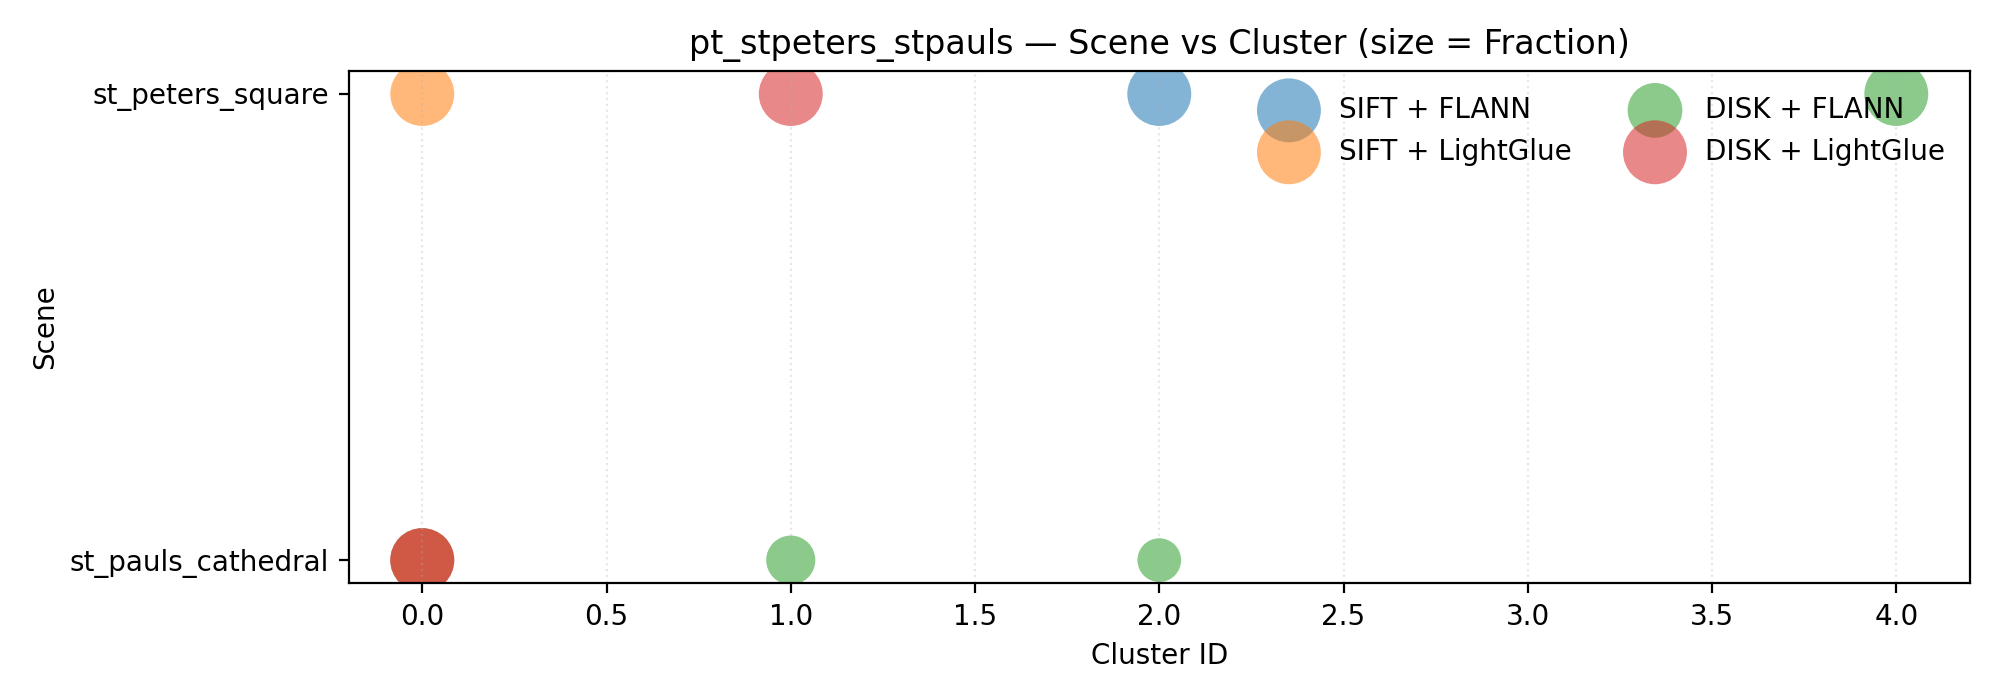
\includegraphics[width=\linewidth]{images/scene_cluster_by_dataset/pt_stpeters_stpauls.png}
            \subcaption{Dataset: pt\_stpeters\_stpauls}
            \label{fig:scene-cluster-A8}
        \end{minipage}

        \begin{minipage}{\textwidth}
            \centering
            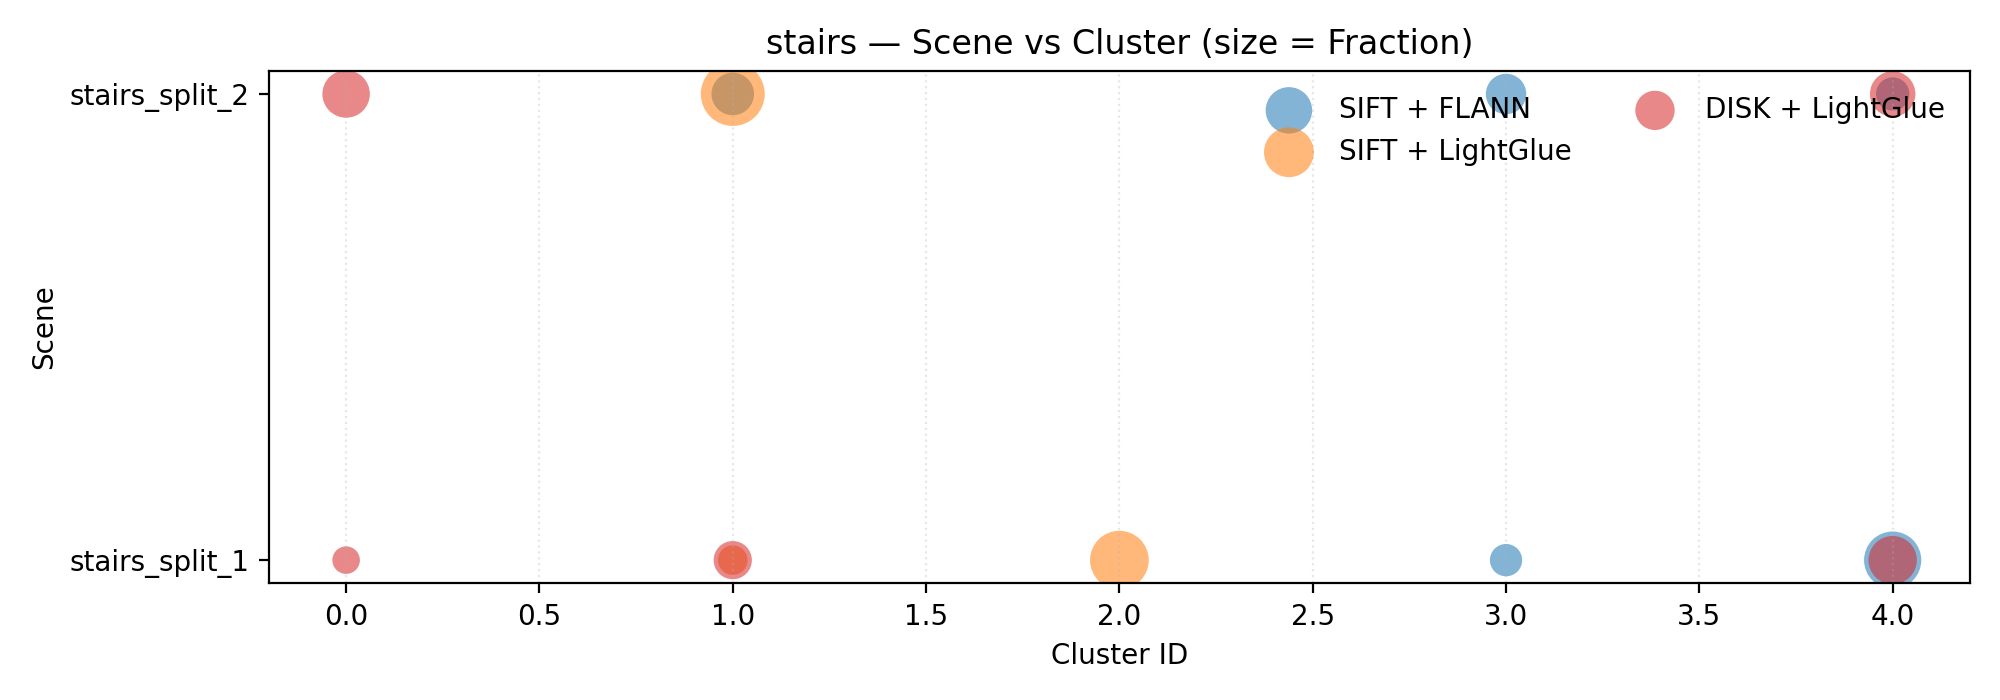
\includegraphics[width=\linewidth]{images/scene_cluster_by_dataset/stairs.png}
            \subcaption{Dataset: stairs}
            \label{fig:scene-cluster-A9}
        \end{minipage}

        \caption{Scene–cluster overlap for the remaining 9 datasets. Each marker at (cluster, scene) encodes overlap size (fraction per scene); color denotes method. Larger, concentrated markers indicate stronger scene–cluster alignment.}
        \label{fig:scene-cluster-9up}
    \end{figure}

    \chapter{Description of AI-Generated Content}\label{appendix:B}
    We use ChatGPT and Gemini-2.5-Flash for language improvement of the report. We also use Claude-3.5 for code generation in evaluation section.
\end{document}
